\section{Results}\label{sec:results}

\subsection{RQ1: What share of migrations come after the shutdown?}

Table~\ref{tab:timing} gives the share of migrations made on or after the shutdown day under each choice of which migrations to count. For OpenAI and Anthropic models shut down by \RetiredBy, so that every model has at least 90 days of data after its shutdown, \AfterLate\% of \AfterLateTotal{} migrations come after the shutdown (95\% CI \AfterLateLow--\AfterLateHigh). Counting every model shut down before our data ends lowers the share to \AfterAll\%, because the most recent shutdowns have had little time to collect late migrations. Counting only migrations from 30 days before the notice onwards, as Kim does, raises it to \AfterWindow\%, because it drops the projects that moved early. Counting only the first migration of each repository away from each model gives \AfterFirst\%. Google, whose shutdown days are only the earliest possible ones, gives \AfterGoogle\%.

Every variant agrees with Kim on the direction: more migrations come after the shutdown than before it. None comes close to Kim's \KimAfterShutdown\% (95\% CI \KimAfterShutdownLow--\KimAfterShutdownHigh), and the intervals do not overlap. Section~\ref{sec:robustness} shows that the gap is not caused by our label: Kim's own rules give \AfterKimLabel\% on our data.

\gentable{timing}{tab:timing}{RQ1: share of migrations made on or after the model's shutdown day, OpenAI and Anthropic unless stated. 95\% Wilson intervals.}

\begin{quote}
\textbf{Answer to RQ1.} Most migrations away from a retired model come after its shutdown, as Kim found, but the share is about \AfterLate\%, not \KimAfterShutdown\%. Between a third and two fifths of projects migrate in time.
\end{quote}

\subsection{RQ2: How long before or after the shutdown do projects migrate?}

Table~\ref{tab:lag} and Figures~\ref{fig:windows} and~\ref{fig:ecdf} show when migrations happen relative to the shutdown. For OpenAI and Anthropic, the median migration comes \ExactDays{} days after the shutdown (95\% CI \ExactDaysLow{} to \ExactDaysHigh), and half of all migrations fall between \ExactDaysQOne{} and \ExactDaysQThree{} days. The busiest window is \ExactPeakWindow{} the shutdown, with \ExactPeakShare\% of migrations. Projects that migrate during the notice period do so when, at the median, \ExactNoticeUsed\% of it has passed.

Late is mostly a little late, but not always. Among migrations made after the shutdown, the median comes \ExactLateDays{} days after it, and the two providers differ: \AnthropicLateDays{} days for Anthropic and \OpenAILateDays{} days for OpenAI. Over all migrations, OpenAI and Anthropic projects migrate at practically the same time (Cliff's $\delta$~=~\CliffAll, $p$~\CliffAllP); among late migrations, OpenAI projects wait clearly longer ($\delta$~=~\CliffLate, \CliffLateSize; Section~\ref{sec:robustness}). Google migrations come a median of \GoogleDays{} days after the earliest possible shutdown day.

\gentable{lag}{tab:lag}{RQ2: days from the shutdown (negative is before). Medians with distribution-free 95\% intervals; ``Notice used'' is the median share of the notice period that had passed, for migrations made during it. Google: from the earliest possible shutdown day.}

\begin{figure}[t]
\centering
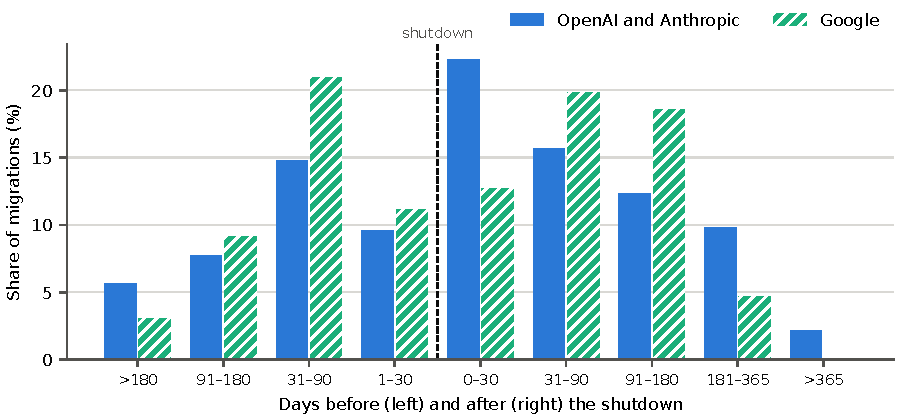
\includegraphics[width=\linewidth]{lag-windows}
\caption{RQ2: share of each provider's migrations in each time window around the shutdown.}\label{fig:windows}
\end{figure}

\begin{figure}[t]
\centering
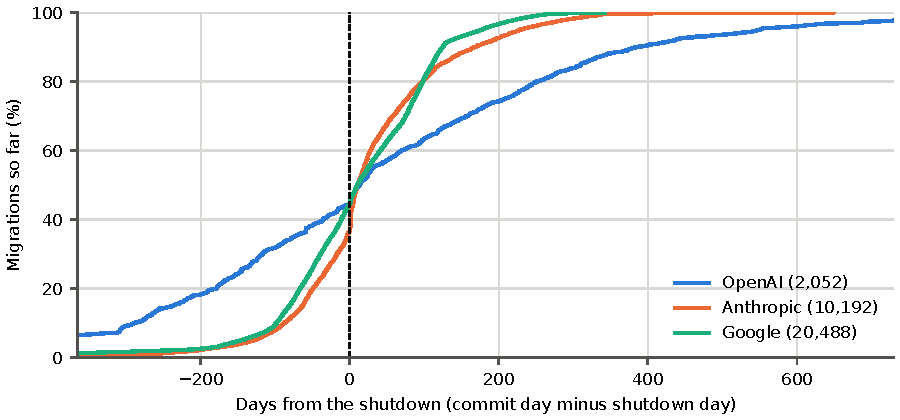
\includegraphics[width=\linewidth]{lag-ecdf}
\caption{RQ2: cumulative share of migrations by days from the shutdown, per provider.}\label{fig:ecdf}
\end{figure}

\begin{quote}
\textbf{Answer to RQ2.} The typical migration comes days after the shutdown, not months: the median is \ExactDays{} days and the busiest month is the one right after the shutdown. Projects that miss the deadline by more than that wait much longer for OpenAI models than for Anthropic ones.
\end{quote}

\subsection{RQ3: What do projects migrate to?}

\TargetFound\% of the \TargetRows{} migrations name the model they move to. Of these, \SameProvider\% stay with the same provider and only \OpenOrOther\% move to an open or other model. Table~\ref{tab:targets} and Figure~\ref{fig:targets} compare the target with the provider's recommended replacement: \FollowsExact\% move to exactly the recommended model, and \FollowsLine\% to it or another model of its line. Most targets are a newer generation of the same series (\GenerationUp\%), but \GenerationDown\% move to an older one. Table~\ref{tab:switches} lists the most common switches.

A fifth of the targets (\TargetOnList\%) are models that are themselves on a provider's retirement list today, so these projects will have to migrate again. \TargetAnnounced\% were already announced for retirement on the day of the commit, and \TargetShutDown\% had already been shut down, mostly Gemini~1.5 models (\TargetShutDownEarlier\% of all targets). \AIAssisted\% of the migrations with a target carry the mark of an AI coding tool, and they are no more likely to move to an older generation than the others.

\gentable{targets}{tab:targets}{RQ3: the target of each migration compared with the provider's recommended replacement, as a share of each provider's migrations.}

\gentable{top-switches}{tab:switches}{RQ3: the ten most common switches.}

\begin{figure}[t]
\centering
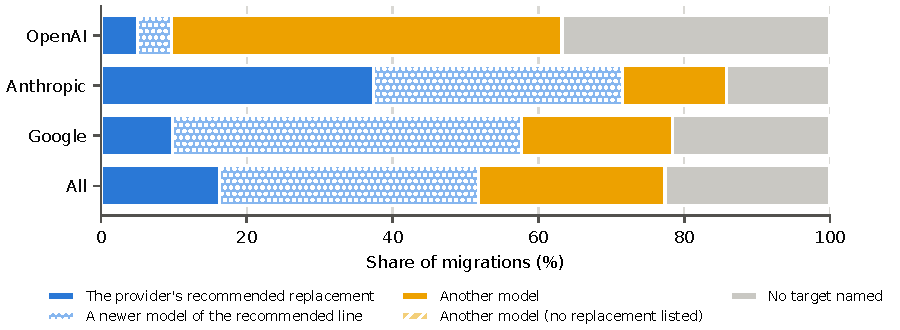
\includegraphics[width=\linewidth]{targets}
\caption{RQ3: how targets relate to the recommended replacement, per provider.}\label{fig:targets}
\end{figure}

\begin{quote}
\textbf{Answer to RQ3.} Projects almost always stay with their provider and mostly follow its recommended line, but one target in five is already scheduled for retirement.
\end{quote}

\subsection{RQ4: Do migration commits change tests or evaluations?}

Table~\ref{tab:files} and Figure~\ref{fig:files} give what the \FilesFound{} sampled migration commits change. \TouchTest\% touch a test file (95\% CI \TouchTestLow--\TouchTestHigh), which matches Kim's \KimTouchTest\%; \AddTest\% add one. Only \TouchEval\% touch an evaluation file, such as a benchmark, golden outputs or an evaluation config (\TouchEvalLow--\TouchEvalHigh). This is a lower bound: by hand we found evaluation changes in \FileHandEval\% of the checked commits. \IdSwap\% of the commits whose diffs we could read change nothing but the model ID. Commits made with an AI coding tool touch tests in \AITouchTest\% of cases and the others in \NotAITouchTest\%, but the intervals overlap.

Kim's \KimMentionEval\% for evaluations counts commit messages that mention an evaluation suite, not files, so it measures something different from our \TouchEval\%.

\gentable{changed-files}{tab:files}{RQ4: what the sampled migration commits change, with 95\% Wilson intervals.}

\begin{figure}[t]
\centering
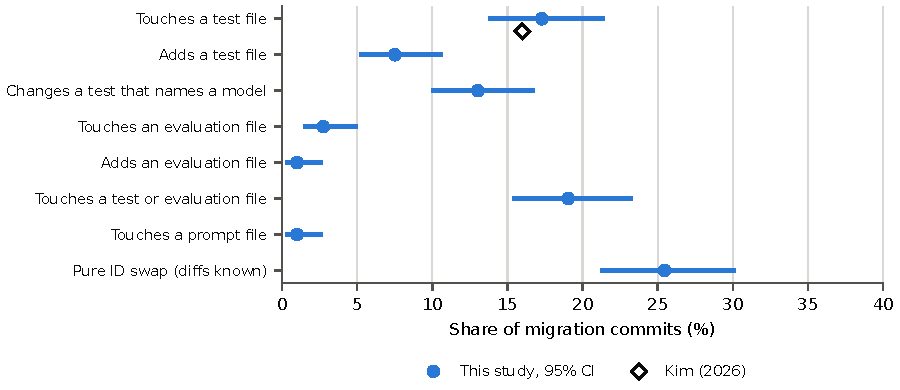
\includegraphics[width=\linewidth]{changed-files}
\caption{RQ4: shares of sampled migration commits with 95\% intervals; the diamond is Kim's \KimTouchTest\%.}\label{fig:files}
\end{figure}

\begin{quote}
\textbf{Answer to RQ4.} About one migration in six touches a test, as Kim found, and very few touch an evaluation. Most projects switch the model without changing the code that would catch a change in its behaviour.
\end{quote}
